\documentclass[tikz,border=6pt]{standalone}

\usepackage{amsmath,amssymb}
\usetikzlibrary{
  arrows.meta,
  positioning,
  calc,
  shapes.geometric,
  shapes.symbols
}

% -------------------- Colors (approx. from reference) --------------------
\definecolor{steelblue}{RGB}{43,101,152}
\definecolor{lightbluebg}{RGB}{229,242,255}

\definecolor{burntorange}{RGB}{198,112,26}
\definecolor{lightorangebg}{RGB}{255,239,224}

\definecolor{deeppurple}{RGB}{106,58,126}
\definecolor{lightpurplebg}{RGB}{244,232,252}

\definecolor{jsongreen}{RGB}{219,240,226}

\begin{document}
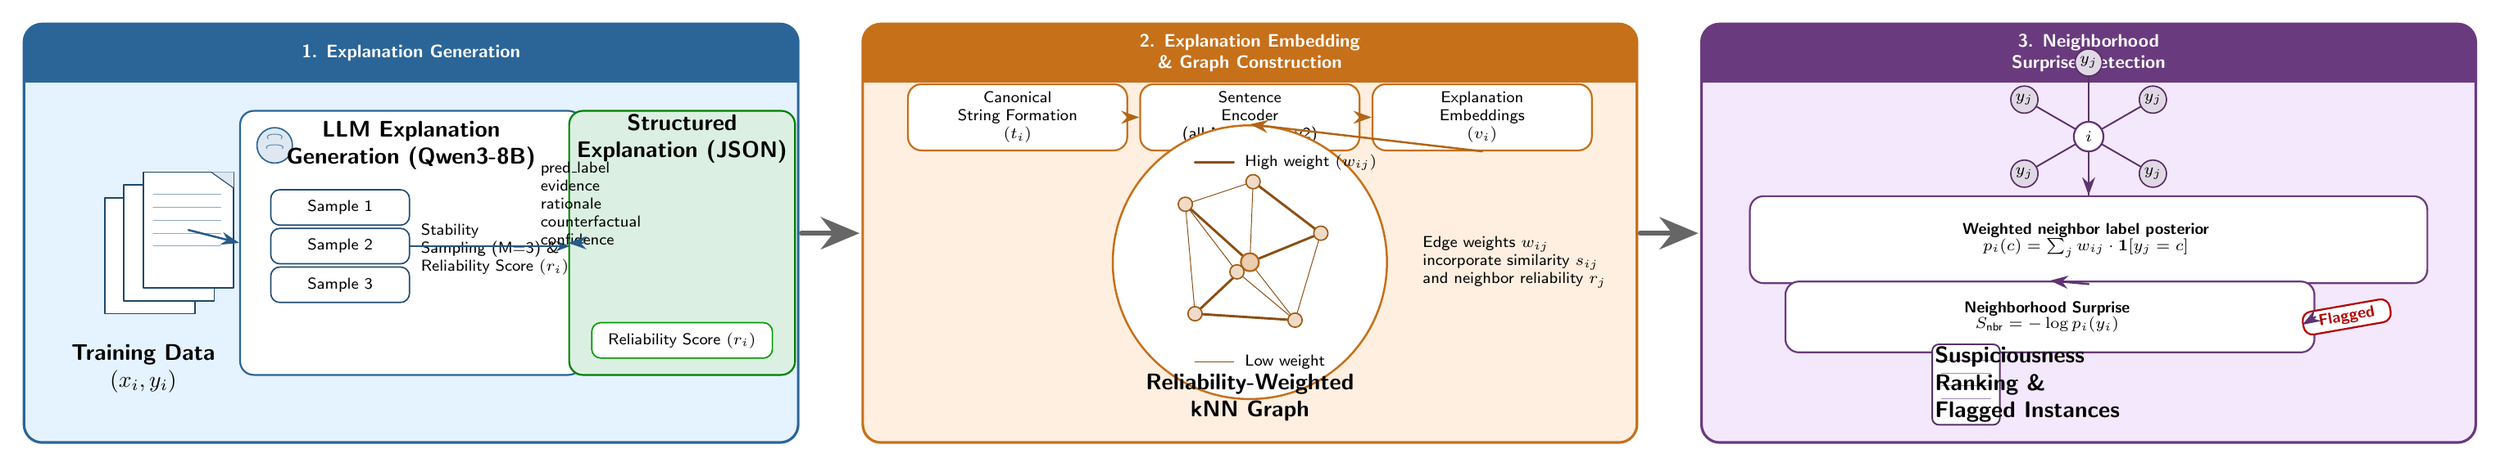
\begin{tikzpicture}[
  x=1cm,y=1cm,
  line cap=round,line join=round,
  >={Stealth},
  every node/.style={font=\sffamily\scriptsize}
]

% -------------------- Global geometry --------------------
\def\panelW{12}
\def\panelH{6.5}
\def\gap{1}
\def\headerH{0.9}

% Panel corners
\coordinate (P1SW) at (0,0);
\coordinate (P1NE) at (\panelW,\panelH);

\coordinate (P2SW) at (\panelW+\gap,0);
\coordinate (P2NE) at (2*\panelW+\gap,\panelH);

\coordinate (P3SW) at (2*\panelW+2*\gap,0);
\coordinate (P3NE) at (3*\panelW+2*\gap,\panelH);

% Header clip SW points
\coordinate (P1HSW) at ($(P1SW)+(0,\panelH-\headerH)$);
\coordinate (P2HSW) at ($(P2SW)+(0,\panelH-\headerH)$);
\coordinate (P3HSW) at ($(P3SW)+(0,\panelH-\headerH)$);

% -------------------- Panel drawing helpers (style) --------------------
\tikzset{
  panelBorder/.style={line width=1.15pt, rounded corners=8pt},
  innerBox/.style={rounded corners=6pt, line width=0.8pt, fill=white},
  smallBox/.style={rounded corners=4pt, line width=0.6pt, fill=white},
  arrowSmall/.style={-{Stealth[length=2.8mm,width=2.0mm]}, line width=0.9pt},
  arrowTiny/.style={-{Stealth[length=2.2mm,width=1.6mm]}, line width=0.7pt},
  arrowBig/.style={-{Stealth[length=6mm,width=5mm]}, line width=2.2pt, draw=black!60}
}

% ==================== PANELS: backgrounds + headers ====================
% ---- Panel 1 ----
\path[draw=steelblue, fill=lightbluebg, panelBorder] (P1SW) rectangle (P1NE);
\begin{scope}
  \clip (P1HSW) rectangle (P1NE);
  \path[fill=steelblue, rounded corners=8pt] (P1SW) rectangle (P1NE);
\end{scope}
\node[font=\sffamily\bfseries\footnotesize, text=white]
  at ($(P1SW)!0.5!(P1NE) + (0,{\panelH/2-\headerH/2})$) {}; % (unused; keeps symmetry)
\node[font=\sffamily\bfseries\footnotesize, text=white]
  at ($(P1HSW)!0.5!(P1NE)$) {1. Explanation Generation};

% ---- Panel 2 ----
\path[draw=burntorange, fill=lightorangebg, panelBorder] (P2SW) rectangle (P2NE);
\begin{scope}
  \clip (P2HSW) rectangle (P2NE);
  \path[fill=burntorange, rounded corners=8pt] (P2SW) rectangle (P2NE);
\end{scope}
\node[font=\sffamily\bfseries\footnotesize, text=white, align=center]
  at ($(P2HSW)!0.5!(P2NE)$) {2. Explanation Embedding\\\& Graph Construction};

% ---- Panel 3 ----
\path[draw=deeppurple, fill=lightpurplebg, panelBorder] (P3SW) rectangle (P3NE);
\begin{scope}
  \clip (P3HSW) rectangle (P3NE);
  \path[fill=deeppurple, rounded corners=8pt] (P3SW) rectangle (P3NE);
\end{scope}
\node[font=\sffamily\bfseries\footnotesize, text=white, align=center]
  at ($(P3HSW)!0.5!(P3NE)$) {3. Neighborhood\\Surprise Detection};

% ==================== PANEL 1: Explanation Generation ====================
% Training data icon (stacked documents - drawn as rectangles with corner fold)
\foreach \xoff/\yoff in {0/0, 0.3/0.2, 0.6/0.4} {
  \fill[white] (1.25+\xoff,2.0+\yoff) rectangle ++(1.4,1.8);
  \draw[steelblue!70!black, line width=0.6pt] (1.25+\xoff,2.0+\yoff) rectangle ++(1.4,1.8);
  % Corner fold
  \fill[steelblue!15] (2.65+\xoff-0.35,3.8+\yoff) -- (2.65+\xoff,3.8+\yoff) -- (2.65+\xoff,3.8+\yoff-0.25) -- cycle;
  \draw[steelblue!70!black, line width=0.4pt] (2.65+\xoff-0.35,3.8+\yoff) -- (2.65+\xoff,3.8+\yoff-0.25);
}
\coordinate (td3) at (2.55,3.3);

% Simple "text lines" on top document
\foreach \yy in {0.55,0.35,0.15,-0.05,-0.25} {
  \draw[steelblue!55, line width=0.35pt]
    ([xshift=-0.55cm,yshift=\yy cm]td3) -- ([xshift=0.50cm,yshift=\yy cm]td3);
}

\node[font=\sffamily\bfseries, align=center] at (1.85,1.15) {Training Data\\$(x_i, y_i)$};

% LLM box
\node[draw=steelblue, innerBox, minimum width=5.3cm, minimum height=4.1cm] (llm) at (6.00,3.10) {};

% Small "brain" icon (simple circular glyph)
\node[draw=steelblue, fill=steelblue!15, circle, line width=0.6pt, minimum size=0.55cm]
  (brain) at ([xshift=0.55cm,yshift=-0.55cm]llm.north west) {};
\draw[steelblue!80, line width=0.35pt]
  ([xshift=-0.10cm,yshift=0.10cm]brain.center) .. controls +(-0.10,0.10) and +(0.10,0.10) .. ([xshift=0.10cm,yshift=0.10cm]brain.center);
\draw[steelblue!80, line width=0.35pt]
  ([xshift=-0.12cm,yshift=-0.05cm]brain.center) .. controls +(-0.08,0.08) and +(0.08,0.08) .. ([xshift=0.12cm,yshift=-0.05cm]brain.center);

\node[font=\sffamily\bfseries, align=center] at ([yshift=-0.55cm]llm.north) {LLM Explanation\\Generation (Qwen3-8B)};

% Sample boxes inside LLM
\node[draw=steelblue!75!black, smallBox, minimum width=2.15cm, minimum height=0.55cm] (s1) at (4.90,3.65) {Sample 1};
\node[draw=steelblue!75!black, smallBox, minimum width=2.15cm, minimum height=0.55cm] (s2) at (4.90,3.05) {Sample 2};
\node[draw=steelblue!75!black, smallBox, minimum width=2.15cm, minimum height=0.55cm] (s3) at (4.90,2.45) {Sample 3};

% Side annotation
\node[align=left] (stab) at (7.30,3.00) {Stability\\Sampling (M=3) \&\\Reliability Score $(r_i)$};
\draw[arrowTiny, draw=steelblue!85!black] (s2.east) -- ([xshift=-0.2cm]llm.east |- s2.east);

% Structured explanation JSON box
\node[draw=green!50!black, fill=jsongreen, rounded corners=6pt, line width=0.8pt,
      minimum width=3.5cm, minimum height=4.1cm] (json) at (10.20,3.10) {};
\node[font=\sffamily\bfseries, align=center] at ([yshift=-0.45cm]json.north) {Structured\\Explanation (JSON)};

\node[align=left] at ([xshift=0.35cm,yshift=-1.45cm]json.north west) {%
  pred\_label\\
  evidence\\
  rationale\\
  counterfactual\\
  confidence
};

\node[draw=green!60!black, fill=white, rounded corners=4pt, line width=0.6pt,
      minimum width=2.8cm, minimum height=0.55cm] (rbox)
  at ([yshift=0.55cm]json.south) {Reliability Score $(r_i)$};

% Internal arrows (Panel 1)
\draw[arrowSmall, draw=steelblue!90!black] (td3.east) -- (llm.west);
\draw[arrowSmall, draw=steelblue!90!black] (llm.east) -- (json.west);

% ==================== PANEL 2: Embedding & Graph Construction ====================
% Top processing pipeline boxes
\node[draw=burntorange, innerBox, minimum width=3.4cm, minimum height=0.85cm, align=center]
  (canon) at (15.40,5.05) {Canonical\\String Formation\\$(t_i)$};

\node[draw=burntorange, innerBox, minimum width=3.4cm, minimum height=0.85cm, align=center]
  (enc) at (19.00,5.05) {Sentence\\Encoder\\(all-MiniLM-L6-v2)};

\node[draw=burntorange, innerBox, minimum width=3.4cm, minimum height=0.85cm, align=center]
  (emb) at (22.60,5.05) {Explanation\\Embeddings\\$(v_i)$};

\draw[arrowSmall, draw=burntorange!90!black] (canon.east) -- (enc.west);
\draw[arrowSmall, draw=burntorange!90!black] (enc.east) -- (emb.west);

% Graph circle
\node[draw=burntorange, fill=white, circle, line width=0.9pt, minimum size=4.25cm]
  (graphCircle) at (19.00,2.80) {};

\coordinate (gC) at (graphCircle.center);
\coordinate (g0) at ($(gC)+(0.00,0.00)$);
\coordinate (g1) at ($(gC)+(-1.00,0.90)$);
\coordinate (g2) at ($(gC)+(0.05,1.25)$);
\coordinate (g3) at ($(gC)+(1.10,0.45)$);
\coordinate (g4) at ($(gC)+(0.70,-0.90)$);
\coordinate (g5) at ($(gC)+(-0.85,-0.80)$);
\coordinate (g6) at ($(gC)+(-0.20,-0.15)$);

% Edge styles (varying thickness = weights)
\tikzset{
  thinEdge/.style={draw=burntorange!70!black, line width=0.35pt},
  thickEdge/.style={draw=burntorange!70!black, line width=1.05pt}
}

% Draw edges first (so nodes sit on top)
\draw[thickEdge] (g0) -- (g1);
\draw[thinEdge]  (g0) -- (g2);
\draw[thickEdge] (g0) -- (g3);
\draw[thinEdge]  (g0) -- (g4);
\draw[thickEdge] (g0) -- (g5);
\draw[thinEdge]  (g0) -- (g6);

\draw[thinEdge]  (g1) -- (g2);
\draw[thickEdge] (g2) -- (g3);
\draw[thinEdge]  (g3) -- (g4);
\draw[thickEdge] (g4) -- (g5);
\draw[thinEdge]  (g5) -- (g1);
\draw[thinEdge]  (g6) -- (g1);
\draw[thinEdge]  (g6) -- (g4);

% Nodes
\tikzset{
  gnode/.style={circle, draw=burntorange!80!black, fill=burntorange!25, line width=0.6pt, minimum size=0.22cm, inner sep=0pt},
  gnodeC/.style={circle, draw=burntorange!90!black, fill=burntorange!35, line width=0.8pt, minimum size=0.28cm, inner sep=0pt}
}
\node[gnodeC] at (g0) {};
\node[gnode]  at (g1) {};
\node[gnode]  at (g2) {};
\node[gnode]  at (g3) {};
\node[gnode]  at (g4) {};
\node[gnode]  at (g5) {};
\node[gnode]  at (g6) {};

% Weight legend inside the circle (high vs low)
\draw[thickEdge] ($(gC)+(-0.85,1.55)$) -- ($(gC)+(-0.25,1.55)$);
\node[anchor=west] at ($(gC)+(-0.20,1.55)$) {High weight $(w_{ij})$};

\draw[thinEdge] ($(gC)+(-0.85,-1.55)$) -- ($(gC)+(-0.25,-1.55)$);
\node[anchor=west] at ($(gC)+(-0.20,-1.55)$) {Low weight};

% Side annotation about edge weights
\node[align=left] at (23.10,2.80) {Edge weights $w_{ij}$\\incorporate similarity $s_{ij}$\\and neighbor reliability $r_j$};

% Arrow from embeddings to graph
\draw[arrowSmall, draw=burntorange!90!black] (emb.south) -- (graphCircle.north);

% Caption
\node[font=\sffamily\bfseries, align=center] at (19.00,0.70) {Reliability-Weighted\\kNN Graph};

% ==================== PANEL 3: Neighborhood Surprise Detection ====================
% Star neighborhood graph (top)
\coordinate (sC) at (32.00,4.75);

\tikzset{
  starNode/.style={circle, draw=deeppurple!80!black, fill=deeppurple!20, line width=0.6pt, minimum size=0.36cm, inner sep=1pt},
  starCenter/.style={circle, draw=deeppurple!90!black, fill=white, line width=0.8pt, minimum size=0.46cm, inner sep=1pt}
}

% Surrounding nodes (edges first, then nodes)
\foreach \ang/\name in {90/a,30/b,-30/c,-90/d,-150/e,150/f} {
  \coordinate (\name) at ($(sC)+(\ang:1.15)$);
}
\foreach \name in {a,b,c,d,e,f} {
  \draw[draw=deeppurple!85!black, line width=0.7pt] (sC) -- (\name);
}

\node[starCenter] (si) at (sC) {$i$};
\foreach \name in {a,b,c,d,e,f} {
  \node[starNode] at (\name) {$y_j$};
}

% Posterior formula box
\node[draw=deeppurple, innerBox, minimum width=10.5cm, minimum height=1.35cm, align=center]
  (post) at (32.00,3.15) {%
    \begin{tabular}{c}
      \bfseries Weighted neighbor label posterior\\[-1pt]
      $p_i(c) = \sum_j w_{ij} \cdot \mathbf{1}[y_j = c]$
    \end{tabular}
  };

% Surprise formula box (leave room on the right for the badge)
\node[draw=deeppurple, innerBox, minimum width=8.2cm, minimum height=1.10cm, align=center]
  (surp) at (31.40,1.95) {%
    \begin{tabular}{c}
      \bfseries Neighborhood Surprise\\[-1pt]
      $S_{\text{nbr}} = -\log p_i(y_i)$
    \end{tabular}
  };

% Connections within panel 3
\draw[arrowSmall, draw=deeppurple!90!black] (si.south) -- (post.north);
\draw[arrowSmall, draw=deeppurple!90!black] (post.south) -- (surp.north);

% "Flagged" badge (stamp-like)
\node[
  draw=red!70!black, fill=white,
  rounded corners=4pt,
  line width=0.8pt,
  font=\sffamily\bfseries\scriptsize,
  text=red!70!black,
  rotate=10,
  inner xsep=7pt, inner ysep=2pt
] (flag) at (36.00,1.95) {Flagged};

\draw[arrowSmall, draw=deeppurple!90!black] (surp.east) -- (flag.west);

% Bottom output label + small list icon
\node[draw=deeppurple!85!black, fill=white, rounded corners=3pt, line width=0.7pt,
      minimum width=1.05cm, minimum height=1.25cm] (outdoc) at (30.10,0.90) {};
\foreach \yy in {0.38,0.18,-0.02,-0.22} {
  \draw[deeppurple!60, line width=0.35pt]
    ([xshift=-0.38cm,yshift=\yy cm]outdoc.center) -- ([xshift=0.38cm,yshift=\yy cm]outdoc.center);
}
\node[font=\sffamily\bfseries, align=left] at (31.05,0.90) {Suspiciousness\\Ranking \&\\Flagged Instances};

% ==================== Cross-panel arrows (large) ====================
% Between panel 1 and 2
\draw[arrowBig] (12.05,3.25) -- (12.95,3.25);
% Between panel 2 and 3
\draw[arrowBig] (25.05,3.25) -- (25.95,3.25);

\end{tikzpicture}
\end{document}

